% Template for PLoS
% Version 3.6 Aug 2022
%
% % % % % % % % % % % % % % % % % % % % % %
%
% -- IMPORTANT NOTE
%
% This template contains comments intended 
% to minimize problems and delays during our production 
% process. Please follow the template instructions
% whenever possible.
%
% % % % % % % % % % % % % % % % % % % % % % % 
%
% Once your paper is accepted for publication, 
% PLEASE REMOVE ALL TRACKED CHANGES in this file 
% and leave only the final text of your manuscript. 
% PLOS recommends the use of latexdiff to track changes during review, as this will help to maintain a clean tex file.
% Visit https://www.ctan.org/pkg/latexdiff?lang=en for info or contact us at latex@plos.org.
%
%
% There are no restrictions on package use within the LaTeX files except that no packages listed in the template may be deleted.
%
% Please do not include colors or graphics in the text.
%
% The manuscript LaTeX source should be contained within a single file (do not use \input, \externaldocument, or similar commands).
%
% % % % % % % % % % % % % % % % % % % % % % %
%
% -- FIGURES AND TABLES
%
% Please include tables/figure captions directly after the paragraph where they are first cited in the text.
%
% DO NOT INCLUDE GRAPHICS IN YOUR MANUSCRIPT
% - Figures should be uploaded separately from your manuscript file. 
% - Figures generated using LaTeX should be extracted and removed from the PDF before submission. 
% - Figures containing multiple panels/subfigures must be combined into one image file before submission.
% For figure citations, please use "Fig" instead of "Figure".
% See http://journals.plos.org/plosone/s/figures for PLOS figure guidelines.
%
% Tables should be cell-based and may not contain:
% - spacing/line breaks within cells to alter layout or alignment
% - do not nest tabular environments (no tabular environments within tabular environments)
% - no graphics or colored text (cell background color/shading OK)
% See http://journals.plos.org/plosone/s/tables for table guidelines.
%
% For tables that exceed the width of the text column, use the adjustwidth environment as illustrated in the example table in text below.
%
% % % % % % % % % % % % % % % % % % % % % % % %
%
% -- EQUATIONS, MATH SYMBOLS, SUBSCRIPTS, AND SUPERSCRIPTS
%
% IMPORTANT
% Below are a few tips to help format your equations and other special characters according to our specifications. For more tips to help reduce the possibility of formatting errors during conversion, please see our LaTeX guidelines at http://journals.plos.org/plosone/s/latex
%
% For inline equations, please be sure to include all portions of an equation in the math environment.  For example, x$^2$ is incorrect; this should be formatted as $x^2$ (or $\mathrm{x}^2$ if the romanized font is desired).
%
% Do not include text that is not math in the math environment. For example, CO2 should be written as CO\textsubscript{2} instead of CO$_2$.
%
% Please add line breaks to long display equations when possible in order to fit size of the column. 
%
% For inline equations, please do not include punctuation (commas, etc) within the math environment unless this is part of the equation.
%
% When adding superscript or subscripts outside of brackets/braces, please group using {}.  For example, change "[U(D,E,\gamma)]^2" to "{[U(D,E,\gamma)]}^2". 
%
% Do not use \cal for caligraphic font.  Instead, use \mathcal{}
%
% % % % % % % % % % % % % % % % % % % % % % % % 
%
% Please contact latex@plos.org with any questions.
%
% % % % % % % % % % % % % % % % % % % % % % % %

\documentclass[10pt,letterpaper]{article}
\usepackage[top=0.85in,left=2.75in,footskip=0.75in]{geometry}

% amsmath and amssymb packages, useful for mathematical formulas and symbols
\usepackage{amsmath,amssymb}

% Use adjustwidth environment to exceed column width (see example table in text)
\usepackage{changepage}

% textcomp package and marvosym package for additional characters
\usepackage{textcomp,marvosym}

% cite package, to clean up citations in the main text. Do not remove.
\usepackage{cite}

% Use nameref to cite supporting information files (see Supporting Information section for more info)
\usepackage{nameref,hyperref}

% line numbers
\usepackage[right]{lineno}

% ligatures disabled
\usepackage[nopatch=eqnum]{microtype}
\DisableLigatures[f]{encoding = *, family = * }

% color can be used to apply background shading to table cells only
\usepackage[table]{xcolor}

% array package and thick rules for tables
\usepackage{array}

\ifndef{SUBMISSION}\usepackage{graphicx}\endif

% create "+" rule type for thick vertical lines
\newcolumntype{+}{!{\vrule width 2pt}}

% create \thickcline for thick horizontal lines of variable length
\newlength\savedwidth
\newcommand\thickcline[1]{%
  \noalign{\global\savedwidth\arrayrulewidth\global\arrayrulewidth 2pt}%
  \cline{#1}%
  \noalign{\vskip\arrayrulewidth}%
  \noalign{\global\arrayrulewidth\savedwidth}%
}

% \thickhline command for thick horizontal lines that span the table
\newcommand\thickhline{\noalign{\global\savedwidth\arrayrulewidth\global\arrayrulewidth 2pt}%
\hline
\noalign{\global\arrayrulewidth\savedwidth}}


% Remove comment for double spacing
%\usepackage{setspace} 
%\doublespacing

% Text layout
\raggedright
\setlength{\parindent}{0.5cm}
\textwidth 5.25in 
\textheight 8.75in

% Bold the 'Figure #' in the caption and separate it from the title/caption with a period
% Captions will be left justified
\usepackage[aboveskip=1pt,labelfont=bf,labelsep=period,justification=raggedright,singlelinecheck=off]{caption}
\renewcommand{\figurename}{Fig}

% Use the PLoS provided BiBTeX style
\bibliographystyle{plos2015}

% Remove brackets from numbering in List of References
\makeatletter
\renewcommand{\@biblabel}[1]{\quad#1.}
\makeatother



% Header and Footer with logo
\usepackage{lastpage,fancyhdr,graphicx}
\usepackage{epstopdf}
%\pagestyle{myheadings}
\pagestyle{fancy}
\fancyhf{}
%\setlength{\headheight}{27.023pt}
%\lhead{\includegraphics[width=2.0in]{PLOS-submission.eps}}
\rfoot{\thepage/\pageref{LastPage}}
\renewcommand{\headrulewidth}{0pt}
\renewcommand{\footrule}{\hrule height 2pt \vspace{2mm}}
\fancyheadoffset[L]{2.25in}
\fancyfootoffset[L]{2.25in}
\lfoot{\today}

%% Include all macros below

\newcommand{\lorem}{{\bf LOREM}}
\newcommand{\ipsum}{{\bf IPSUM}}

%% User macros

\renewcommand{\equationautorefname}{Eq.}
\renewcommand{\tableautorefname}{Tab.}
\def\R{\mathbb R}
\def\RR{\R^2}
\def\Rp{\R^p}
\def\d{\mathrm d}
\def\Jab{\tilde J_{\alpha\beta}}
\def\Fab{\tilde F_{\alpha\beta}}
\def\Gab{\tilde G_{\alpha\beta}}
\def\Jij{J_{ij}}
\def\Fij{F_{ij}}
\def\gij{G_{ij}}
\def\wu{w_\textrm{U}}
\def\hu{h_\textrm{U}}
\def\bO{\mathcal{O}}
\def\CDF{\mathrm{CDF}}
\newcommand{\avg}[1]{\langle{#1}\rangle}
\newcommand{\norm}[1]{\lVert{#1}\rVert}
% \def\avg#1{\langle{#1}\rangle}
\renewcommand{\vec}[1]{\boldsymbol{#1}}

%% END MACROS SECTION


\begin{document}
\vspace*{0.2in}

% Title must be 250 characters or less.
\begin{flushleft}
% TODO: what title is better ?
% \title{Equivalence of neural field dynamics with different embedding dimensionality}
% \title{Neural fields with different embedding dimensionality can express identical dynamics}
% \title{Neural dynamics can be equivalently embedded in neural fields of different dimensions}
{\Large
\textbf\newline{Neural fields with different embedding dimensionality can express identical dynamics} % Please use "sentence case" for title and headings (capitalize only the first word in a title (or heading), the first word in a subtitle (or subheading), and any proper nouns).
}
\newline
% Insert author names, affiliations and corresponding author email (do not include titles, positions, or degrees).
\\
Nicole Vadot\textsuperscript{1},
Valentin Schmutz\textsuperscript{1},
Wulfram Gerstner\textsubscript{1}
% Name1 Surname\textsuperscript{1,2\Yinyang},
% Name2 Surname\textsuperscript{2\Yinyang},
% Name3 Surname\textsuperscript{2,3\textcurrency},
% Name4 Surname\textsuperscript{2},
% Name5 Surname\textsuperscript{2\ddag},
% Name6 Surname\textsuperscript{2\ddag},
% Name7 Surname\textsuperscript{1,2,3*},
% with the Lorem Ipsum Consortium\textsuperscript{\textpilcrow}
\\
\bigskip
\textbf{1} LCN, EPFL, Lausanne, Vaud, Switzerland
% \\
% \textbf{2} Affiliation Dept/Program/Center, Institution Name, City, State, Country
% \\
% \textbf{3} Affiliation Dept/Program/Center, Institution Name, City, State, Country
% \\
\bigskip

% Insert additional author notes using the symbols described below. Insert symbol callouts after author names as necessary.
% 
% Remove or comment out the author notes below if they aren't used.
%
% Primary Equal Contribution Note
% \Yinyang These authors contributed equally to this work.

% Additional Equal Contribution Note
% Also use this double-dagger symbol for special authorship notes, such as senior authorship.
% \ddag These authors also contributed equally to this work.

% Current address notes
% \textcurrency Current Address: Dept/Program/Center, Institution Name, City, State, Country % change symbol to "\textcurrency a" if more than one current address note
% \textcurrency b Insert second current address 
% \textcurrency c Insert third current address

% Deceased author note
% \dag Deceased

% Group/Consortium Author Note
% \textpilcrow Membership list can be found in the Acknowledgments section.

% Use the asterisk to denote corresponding authorship and provide email address in note below.
% * correspondingauthor@institute.edu

\end{flushleft}
% Please keep the abstract below 300 words
\section*{Abstract}

\ifndef{SUBMISSION}
\includegraphics[width=\textwidth]{../figures/cover.pdf}
\endif

Classical neural field models describe interactions between neurons positioned in an embedding; often a physical space (for instance, that of the cortical sheet) or, later, abstract spaces (for instance, that of neuron celltypes), in which the dynamics are highly regular in space and time. Recent improvements in recordings of neural activity have further demonstrated the smoothness of the neural dynamics, when placed in an appropriate embedding space.

Decoupling the embedding space from the physical position of neurons begs the question of uniqueness of the embedding space. Given an embedding space and neural dynamics theron, are there other embedding spaces which can express the same behavior?

We show that embedding spaces are not unique, and more suprisingly, that we can find multiple embedding spaces in different dimensions, which all model identical neural dynamics.
The core of this work lies in the study of bijective mappings $S$ between $[0,1]^2$ and $[0,1]$, which allows mapping a two-dimensional neural field to an equivalent one-dimensional neural field.
This procedure is easily generalized to map between embeddings in arbitrary number of dimensions.
We introduce a measure of locality, which quantifies how the regularity of the neural fields in conserved through the mappings $S$. This allows us to show that the resulting neural field is well-behaved, and can therefore be approximated using classical grid-based methods.
To illustrate these results through numerical models, we describe a coarse-graining procedure enforcing the locality of the numerically applied mappings.

% Please keep the Author Summary between 150 and 200 words
% Use first person. PLOS ONE authors please skip this step. 
% Author Summary not valid for PLOS ONE submissions.   
\section*{Author summary}
[TODO?]
\linenumbers


\section{Introduction}

% NOTE: the goal here is to give an intuitive understanding of the problem,
% kind of in the same "story-telling"-way that I did in the master thesis.
% This also allows to introduce some of the notation that I use later on.

% \subsection{Neural field models in neuroscience}

Early recordings of cats' somatosensory \cite{Mou57} and visual \cite{HubWie62} cortices suggested that the cortical sheet is organized in vertical columns of functionally similar neurons.

The columnar organization of the cortex motivated the design of spatially structured models of neural population dynamics, namely neural field models \cite{WilCow73,Nun74,Ama77}, where the spatial dimensions corresponded to the two dimensions of the cortical sheet. 

As models of spatiotemporal neural population dynamics on the cortical sheet, neural field models can be used to explain experimentally observed patterns of cortical activity, such as travelling waves in visual \cite{SatNau12,MulRey14}, somatosensory \cite{PetHah03,FerBol06}, motor \cite{RubRob06,TakKim15}, and hippocampal \cite{LubSia09,PatFuj12,PatSch13} cortices (see \cite{MulCha18} for a review), and are used to model large-scale brain signals, such as electroencephalography (EEG) recordings \cite{Bre17} (see also \cite{DipRan18} for an example of neural field modelling of calcium imaging recording of the visual cortex).

More recent recording methods, especially in rodents, have provided evidence of low-dimensional organization of neuronal activity that does not depend on the physical locations of neurons on the cortical sheet. For example, contrary to cats' visual cortex, the orientation selectivity of pyramidal neurons in a rat's visual cortex does not depend on their locations, that is, orientation selectivity is heterogeneous at any given location \cite{OhkChu05}. Moreover, the activity of interneurons in any small volume of the visual cortex is also heterogeneous and seems to be structured by a low-dimensional manifold of fine cell subtypes \cite{BugDuf22}. The local functional heterogeneity of neuronal activity in the cortex challenges the old concept of functionally homogeneous cortical columns and, with it, classical neural field models. 

While, historically, the spatial dimensions in neural field models have been the two dimensions of the cortical sheet (with the notable exception of the ring models for orientation selectivity in the visual cortex \cite{BenBar95} and the head-direction system \cite{Zha96}), the ``space'' in neural field models does not need to represent physical space but can represent any suitable abstract embedding space. Neural field models with abstract embedding spaces could constitute a generalization of classical neural field theory for cortical networks that are not solely structured by distances of neurons on the cortical sheet.

Moreover, this work is motivated by recent mathematical developments \cite{JabPoy21} in mean-field theories involving the theory of graphons. Informally, these results suggest that, as long as the connectivity scales as $1/N$ (where $N$ is the number of neurons), the dynamics of large networks can be described in the $N \to \infty$ limit by a neural field equation where the embedding is simply the interval $[0,1]$. The main contribution of this paper is the derivation of a method, allowing to explicitly write such a one-dimensional neural field, starting from a known higher-dimensional neural field.

% \subsection{Formulating a one-dimensional neural field}

% If we consider neural fields in abstract embedding spaces, which embedding space should we choose? More fundamentally, given some spatiotemporal dynamics, is there a "natural" choice for the embedding space?

% We show that the answer to the second question is highly nontrivial because even the dimensionality of the embedding space, for some given spatiotemporal dynamics, is not clearly defined. This means that it is possible to find two embeddings (each associated with a connectivity kernel) of different dimensions that give rise to identical dynamics.

% TODO: do we talk about the tau=1, R=1 ?
% TODO: do we talk about external currents ?

We begin our work by considering a neural field associated with a $p$-dimensional embedding $\Rp$. $h(\vec z, t)$ describes the potential of the neural population at position $\vec z=(z_1,\cdots,z_p)$ in the embedding. The connectivity kernel $w(\vec y, \vec z)$ describes the amplitude of the recurrent currents from the population at $\vec z$ to the population at $\vec y$. Importantly, $w(\vec y, \vec z)$ is a ``smooth'' function in both arguments. This is a natural consequence of the derivation of neural field equations (rigorous proofs of convergence of networks to neural fields are still an active area of study, and we may cite \cite{CheDua19,AGATHENERINE202286} for recent developments).
$\rho(\vec z)$ measures the number of neurons per unit volume of the embedding space, effectively weighing the recurrent currents. The monotonic increasing activation function $\phi(h)$ describes the firing rate of a given neuron (population) with potential $h$. The neural field then evolves according to \autoref{eq:nf-in-rp}:  

\begin{equation} \label{eq:nf-in-rp}
\partial_t h(\vec z, t) = \underbrace{-h(\vec z, t)}_\text{exponential decay} + \underbrace{\int_{\mathbb{R}^p} w(\vec z, \vec y) \phi(h(\vec y, t)) \rho(\vec y) \mathrm d \vec y}_\text{recurrent current}.
\end{equation}

Without loss of generality, a simple bijective mapping can be applied to reduce any $p$-dimensional neural field to a neural field on $[0,1]^p$. Additionally redefining the connectivity kernel to absorb the density and determinant of the transformation (see an example in section 2.5 of \cite{nvadot2023mathesis}), we arrive at \autoref{eq:nf-in-01p}, a general form for any neural field equation in $p$ dimensions:

% The embedding space $\Rp$ (or any $p$-dimensional space) can be mapped to $[0,1]^p$ via bijective functions between the two spaces. For instance, if the neuron density factorizes as $\rho(z_1, \cdots, z_p)= \rho_1(z_1) \cdots \rho_p(z_p)$, then the associated cumulative density functions can be used to perform a change of variables, resulting in the an equivalent "uniform" neural field equation:

\begin{equation} \label{eq:nf-in-01p}
\partial_t h_U(t, \vec v) = -h_U(t, \vec v) + \int_{[0,1]^p} w_U(\vec v, \vec u) \phi(h_U(t, \vec u)) \mathrm d \vec u.
\end{equation}

This form highlights the central role of the connectivity kernel $w_U$, which together with the initial condition $h_U(t=0, \vec v)$, uniquely determines the neural dynamics.

% If the neuron density does not factorize, then one can arrive at the same formulation by redefining the connectivity kernel to include the neuron density and the determinant of the transformation. [TODO: this sentence might need some work]

In particular for $p=2$, we show that for any two-dimensional neural field equation (that is, with two spatial dimensions), there is a one-dimensional neural field equation (where the embedding space is simply the interval $[0,1]$), from which the solution to the two-dimensional equation can be fully reconstructed. The mapping from the two-dimensional equation to the one-dimensional equation is done via well-known measurable bijections between the square $[0,1]^2$ and the interval $[0,1]$. Importantly, these bijections are not diffeomorphisms.
% Also, we show that although the connectivity kernel of the one-dimensional equation seems to have a fractal structure, it is sufficiently regular for its solution to be numerically approximated using standard grid-based simulations.
The main idea is to define a measurable bijective mapping $S : [0,1]^2 \mapsto [0,1]$ and a measure $\lambda : [0,1]^2 \mapsto \mathbb{R}^+$, such that we can write a one-dimensional neural field	$\tilde h(\alpha, t)$ with a connectivity kernel defined as $\tilde w(\alpha, \beta) = w_U(S^{-1}(\alpha), S^{-1}(\beta))$. Doing this, we arrive at the following one-dimensional neural field equation: 
% The question of well-posedness of the neural field in \autoref{eq:nf-in-01} is defered in \autoref{sec:proof-equivalence}.

\begin{equation} \label{eq:nf-in-01}
\partial_t \tilde h(\alpha, t) = -\tilde h(\alpha, t) + \int_{[0,1]} \tilde w(\alpha, \beta) \phi(\tilde h(\beta, t)) \left[\lambda \circ S^{-1}\right](\d \beta).
\end{equation}

The difficulty in writing the one-dimensional neural field, is that the spatial structure of the original neural field in $[0,1]^2$ may be lost.
Fig. [TODO] illustrates this problem: if the mapping is seemingly random, the regularity of the orginal neural field is destroyed. Contrarily, if the mapping is ``local'', the resulting neural field might still be well-defined and exhibit identical dynamics, despite the apparent discontinuities.
The intuition is that we would like populations close in $[0,1]^2$ to be bijectively mapped to populations close in $[0,1]$. However, since $S^{-1}$ is a bijection, it cannot, by Netto's theorem, also be continuous. The core of our argument lies in the fact that we can relax the requirement that the spatial embedding is continuous, instead, we only require it is ``continuous on average''. We quantify this by introducing the ``locality'' $V(S^{-1})$ of the mapping $S^{-1}$, which measures if small neighbourhoods in $[0,1]$ are mapped to small neighbourhoods in $[0,1]^2$. Using locality, we then prove that the mean-field approximation is still valid, implying that we can simulate the one-dimensional neural field using classical grid-based methods.

\ifndef{SUBMISSION}
\includegraphics[height=15em]{../figures/locality.png}

[TODO: clean up this graphic, cite it in text. we need to introduce a random mapping maybe ?]
\endif

% question of uniqueness, discretization error, mean field limit and locality, link with numerical simualtions. chap 1.4, chap 3.1

% "discretization error"

% chap 1.1, chap 2.1, 2.5

Our results suggest that the notion of spatial dimensionality in neural field dynamics is not well-defined if not associated with a constraint on the regularity of the neural fields (and the connectivity kernel). Thereby, by studying a simple toy model, this work illustrates the importance of the analytic notion of regularity when neural population dynamics over abstract continuous spaces are considered. 

\section{Mappings $S$ from $[0,1]^2$ to $[0,1]$}

\subsection{Motivation for a grid-based approach} \label{sec:grid-motivation}

We motivate the upcoming study of the mappings $S$ by considering a grid discretization of the original two-dimensional space $[0,1]^2$. For this, we subdivide each axis into $2^n$ equal segments (each segment has a length of $2^{-n}$), where $n \in \mathbb{N}$ describes the grid resolution. This results in a grid constituted of $2^n \times 2^n = 4^n$ squares in $[0,1]^2$. To each square bin indexed $i \in \{1,\cdots,4^n\}$, we associate a position $\vec{v_i^{(n)}} = (v_{i,1}^{(n)}, v_{i,2}^{(n)})$ located at the origin of the bin. Since everytime $n$ is incremented by one, every axis is subdivided into two smaller equal parts, the positions $v_{i,1}^{(n)}$ and $v_{i,2}^{(n)}$ naturally lend themselves to a binary notation.

For the component $v_\mu \in [0,1]$ of an arbitrary position $\vec{v} \in [0,1]^2$, we introduce $v_\mu^{(n)}$ to denote its $n$-bit truncation, where $\mu = 1,2$ (and in general for $p$-dimensional grids, $\mu=1, \cdots, p$) indicates the axis of the dimension. Additionally, we write the error of the trunctation as a small corrective factor $0 \leq c^{(n)} < 2^{-n}$. In bit notation, this yields: 

\begin{equation} \begin{aligned} \label{eq:positions-v}
v_1 &= v_1^{(n)} + c_1^{(n)} = \sum_{l=1}^n b_1^l 2^{-l} + c_1^{(n)} = 0.b_1^1 b_1^2 \cdots b_1^n + c_1^{(n)}, \\
v_2 &= v_2^{(n)} + c_2^{(n)} = \sum_{l=1}^n b_2^l 2^{-l} + c_2^{(n)} = 0.b_2^1 b_2^2 \cdots b_2^n + c_2^{(n)}.
\end{aligned}\end{equation}

Since $c_\mu^{(n)} < 2^n$, it can easily be seen that $v_\mu^{(n)} \to v_\mu$ as $n\to\infty$, that is, as we take finer and finer grids, the truncation tends to the true value of $\vec{v}$. In general, the bits of the component $v_\mu$ can be expressed as:

\begin{equation*}
b_\mu^l = \mathrm{Ind} \left\{ 2^{l-1}v_\mu - \left\lfloor 2^{l-1}v_\mu \right\rfloor \right\}
\end{equation*}

Sampling the original connectivity kernel at the grid points $\vec{v_i}$ and $\vec{u_j}$ yields a numerical connectivity matrix $J_{ij} := w_U(\vec{v_i}, \vec{u_j})$, illustrated in Fig. [TODO], which can be used to simulate the resulting population dynamics equation:

\begin{equation} \label{eq:population-dynamics}
\frac{\d}{\d t} h_i(t) = -h_i(t) + \sum_{j=1}^{4^n} J_{ij} \phi(h_j(t)), \quad \text{for all } i \in \{1,\cdots,4^n\}.
\end{equation}

\ifndef{SUBMISSION}
\includegraphics[height=20em]{../figures/discretization.png}

[TODO: the discretization here and the sampling on a grid, and the limit of n to infty. do we need to clarify explicitly the bounds of each square bin ?]
\endif

\autoref{eq:population-dynamics} can be seen as the discretized version of \autoref{eq:nf-in-01p}, where we associate $h_i(t) := h_U(\vec{v_i}, t)$. Indeed, by a mean-field argument on the original smooth neural field, the discrete dynamics converge to the true solution of the neural field, because the error of the mean-field approximation in $[0,1]^2$ vanishes as we take finer grids, letting $n \to \infty$.

We would now like to derive a bijective mapping $S$, such that the same argument applies on the neural field in $[0,1]$. Intuively, we want $S$ to conserve the regularity of the neural field on $[0,1]^2$, since if the mean-field argument also carries over to the one-dimensional neural field, it seems natural that it will express identical dynamics.

\subsection{$S$ as the pointwise limit of a sequence of bijections $S^n$}

Let us define a sequence of bijective mappings $\{S^n\}_{n \in \mathbb N}$, acting on the $n$-bit truncations $\vec{v^{(n)}}$ of any $\vec{v} \in [0,1]^2$, as well as the corresponding sequence of images $\{\alpha^n := S^n(\vec{v^{(n)}})\}_{n \in \mathbb N}$. $S^n$ defines the following bijection between points on the two-dimensional and one-dimensional grids:

\begin{equation} \label{eq:def-S} \begin{aligned}
S^n :& \{\tfrac{l-1}{2^n}\;|\;l\in\{1,\cdots,2^n\}\}^2 \mapsto \{\tfrac{i-1}{4^n}\;|\;i\in\{1,\cdots,4^n\}\},\\
\text{such that }&(v_1^{(n)}, v_2^{(n)}) = (0.b_1^1 b_1^2 \cdots b_1^n, 0.b_2^1 b_2^2 \cdots b_2^n) \mapsto \alpha^n = 0.b^1 b^2 \cdots b^{2n}.
\end{aligned} \end{equation}

% NOTE: it is important to write \alpha^n, and not \alpha^{(n)}, since in all generality the n-bit trunction of \alpha is NOT equal to \alpha^n (example: the column mapping \alpha^n = C(v))

We write $\alpha^n$ using the $2n$ bits $\{b^1, b^2, \cdots, b^{2n}\}$, which is intuitively the lowest number of bits required so that $S^n$ remains a bijection, since it takes $2n$ bits of information as argument. More than $2n$ bits could be allowed while maintaining bijectivity, but we omit this possibility, since they wouldn't strictly be required. In this formulation, it becomes clear that in order to be a bijection, every bit of the input must be used once and only once to form the image. Setting aside bit inversions, this means that we let $S^n$ define a permutation of the $2n$ input bits. [TODO: are more details necessary ? I think this is clear enough, though in the thesis manuscript I got over this point in more detail]

For any finite $n$ and any $(v_1,v_2) \in [0,1]^2$, we may extend the definition of $S^n$ with $S^n(v_1, v_2) := S^n(v_1^{(n)}, v_2^{(n)})$ such that it acts on the entire space $[0,1]^2$ instead of the finite set of grid points. While this extension is obviously not bijective (all points in a grid cell are ``rounded'' to the corresponding grid position), in the $n \to \infty$ limit the finite-$n$ truncation converges, such that the pointwise limit could still be a bijection. In \autoref{sec:mapping-examples} we formulate two examples, where in one case the extension converges to a bijection, and in the other it doesn't.

Given $(v_1, v_2) \in [0,1]^2$ and the sequence $\{S^n(v_1, v_2)\}_{n \in \mathbb N}$, we then we define $\alpha = S(v_1, v_2)$ as its limit, if it exists. Informally, pointwise convergence of $\{S^n\}_{n\in\mathbb N}$ requires that the least signficiant bits of the input be mapped to the least significant bits of the image, ensuring that small corrections in the input $\vec{v}$ result in small corrections in the image $\alpha$.

To illustrate this, let us give an example of the sequence $\{A^n\}_{n \in \mathbb N}$ that does not converge pointwise:

\begin{equation*}
\alpha_A^n = A^n(v_1^{(n)},v_2^{(n)}) = 0.b_1^n b_2^n b_1^{n-1} b_2^{n-1} \cdots b_1^1 b_2^1 = \sum_{k=1}^n b_1^{n+1-k} 2^{1-2k} + b_2^{n+1-k} 2^{-2k}.
\end{equation*}

The permutation between the bits of $\alpha^n$, and the bits of $(v_1^{(n)}, v_2^{(n)})$ is illustrated in Fig. [TODO: arrow connecting the bits together], and shows how this example does not respect the bit ordering described previously.
For finite $n$, $A^n$ is clearly bijective and has a well-defined inverse $A^n_\textrm{inv}$:

\begin{equation*} \begin{aligned}
v_1^{(n)} &= A^n_{\textrm{inv},1}(\alpha^n) = 0.b_A^{2n-1} b_A^{2n-3} \cdots b_A^1 = \sum_{k=1}^n b_A^{2(n-k)-1} 2^{-k}, \\
v_2^{(n)} &= A^n_{\textrm{inv},2}(\alpha^n) = 0.b_A^{2n} b_A^{2n-2} \cdots b_A^2 = \sum_{k=1}^n b_A^{2(n+1-k)} 2^{-k}.
\end{aligned} \end{equation*}

However, for any $(v_1,v_2)$, the sequence $\{A^n(v_1, v_2)\}_{n \in \mathbb N}$ does not converge. In Fig. [TODO] we graph the mapping $A^n$, which demonstrates that the image of any point $(v_1,v_2)$ in $[0,1]^2$ diverges as $n$ increases. As $n$ increases, $A^n$ ``refines'' its input with fluctuations of order $2^{-n}$ (because it works with truncations of $(v_1, v_2)$, which have error $c^{(n)} < 2^{-n}$), but the image $\alpha^n=b_1^n 2^{-1} + b_2^n 2^{-2} + b_1^{n-1} 2^{-3} + b_2^{n-1} 2^{-4} \cdots$ fluctuates (at least) with fixed amplitude $\sim 2^{-2}$, independantly of $n$. Therefore the image never converges, and $\{A_n\}_{n \in \mathbb N}$ is not pointwise convergent.

\ifndef{SUBMISSION}
\includegraphics[width=\linewidth]{../figures/mapping-A.pdf}
[TODO: remove the numbers on this figure, dot the grid nodes]
\endif

Within the context of sequences of mappings acting as permutations on the bits of continually refined grid points, the criterion of pointwise convergence restricts the general ``form'' that those mappings can take.
In the following section, we give the standard examples of the Column and the Z-mapping, showing that our formulation is flexible enough to express mappings that have good properties such as ``locality'', while being simple enough to help build intuitions.


\subsection{Two examples of sequences of mappings: the Column and the Z-mapping} \label{sec:mapping-examples}

Let us provide two examples of sequence of mappings that are pointwise convergent, and act as permutation of the grid point bits.
We first define the sequence of Column mappings $\{C^n\}_{n\in\mathbb N}$ as the concatenation of the input bits of $v_1^{(n)}$, followed by the bits of $v_2^{(n)}$. We define the image $\alpha_C^n = 0.b_C^1 b_C^2 \cdots b_C^{2n}$ as:

\begin{equation} \label{eq:def-column-mapping}
\alpha_C^n := C^n(v_1^{(n)}, v_2^{(n)}) = 0.b_1^1 b_1^2 \cdots b_1^n b_2^1 b_2^2 \cdots b_2^n = \sum_{k=1}^n b_1^k 2^{-k} + b_2^k 2^{-(k+n)}.
\end{equation}

Instead of concatenation, we may also interleave the bits of $v_1^{(n)}$ and $v_2^{(n)}$, defining the sequence of Z-mappings $\{Z^n\}_{n\in\mathbb N}$. We define the image $\alpha_Z^n = 0.b_Z^1 b_Z^2 \cdots b_Z^{2n}$ as:

\begin{equation} \label{eq:def-z-mapping}
\alpha_Z^n := Z^n(v_1^{(n)}, v_2^{(n)}) = 0.b_1^1 b_2^1 b_1^2 b_2^2 \cdots b_1^n b_2^n = \sum_{k=1}^n b_1^k 2^{1-2k} + b_2^k 2^{-2k}.
\end{equation}

We graph both mappings in Fig. [TODO]. At finite $n$, both mappings can be inversed to retrieve the truncations:

\begin{equation} \begin{aligned}
C^n_{\textrm{inv},1}(\alpha_C^n) &= 0.b_C^1 b_C^2 \cdots b_C^n = \sum_{k=1}^n b_C^k 2^{-k} = v_1^{(n)}, \\
C^n_{\textrm{inv},2}(\alpha_C^n) &= 0.b_C^{n+1} b_C^{n+2} \cdots b_C^{2n} = \sum_{k=1}^n b_C^{n+k} 2^{-k} = v_2^{(n)}, \\
Z^n_{\textrm{inv},1}(\alpha_Z^n) &= 0.b_Z^1 b_Z^3 \cdots b_Z^{2n-1} = \sum_{k=1}^n b_Z^{2k-1} 2^{-k} = v_1^{(n)},\\
Z^n_{\textrm{inv},2}(\alpha_Z^n) &= 0.b_Z^2 b_Z^4 \cdots b_Z^{2n} = \sum_{k=1}^n b_Z^{2k} 2^{-k} = v_2^{(n)}.
\end{aligned} \end{equation}

\ifndef{SUBMISSION}
\includegraphics[height=20em]{../figures/mapping-col-Z.pdf}

[TODO: add labels, show n=3, etc. Comment on the recursive and fractal structure of the Z-mapping, and the projection for the Column mapping.]
\endif

Both mappings converge pointwise, since for any $(v_1,v_2) \in [0,1]^2$, the limit exists, which we write as $C(v_1,v_2)$ and $Z(v_1,v_2)$ respectively, and we may find the following upper bounds:

\begin{equation} \begin{aligned}
& C(v_1,v_2) = \sum_{k=1}^\infty b_1^k 2^{-k} = v_1, \;\text{and}\; |C^n(v_1,v_2)-C(v_1,v_2)| \leq 2^{-n},\\
& Z(v_1,v_2) = \sum_{k=1}^\infty b_1^k 2^{-k} + b_2^k 2^{-(k+n)}, \;\text{and}\; |Z^n(v_1,v_2)-Z(v_1,v_2)|\leq 2^{-(2n-1)}.
\end{aligned} \end{equation}

Importantly, the limit $C(v_1,v_2)=v_1$ is a projection, and is therefore not bijective. This result is not suprising, since in the definition of $C^n$ (\autoref{eq:def-column-mapping}) the information on the bits of $v_2$ appears only after the bit $n$, and gets discarded in the $n \to \infty$ limit. The Z-mapping does not suffer from the same problem, since informally the most significant bits of the input get mapped to the most significant bits of the image (no information gets lost), and we can conveniently take the $n \to \infty$ limit of $Z_{\textrm{inv},1}^n$ and $Z_{\textrm{inv},2}^n$:

\begin{equation} \begin{aligned}
&Z_{\textrm{inv,1}}^n(\alpha^n) \xrightarrow{n \to \infty} Z^{-1}_1(\alpha) = 0.b_Z^1 b_Z^3 \cdots = \sum_{k=1}^\infty b_Z^{2k-1} 2^{-k} = v_1,\\
&Z_{\textrm{inv,2}}^n(\alpha^n) \xrightarrow{n \to \infty} Z^{-1}_2(\alpha) = 0.b_Z^2 b_Z^4 \cdots = \sum_{k=1}^\infty b_Z^{2k} 2^{-k} = v_2.
\end{aligned} \end{equation}

\section{Numerical simulations of mappings from two-dimensional to one-dimensional neural fields}

In the interest of developing an insight on the properties of the two mappings introduced previously, let us now develop a numerical grid-based simulation.
As established in the \autoref{sec:grid-motivation}, the original two-dimensional neural field can be simulated by sampling the connectivity kernel at pairs of discrete grid points $(\vec{v_i},\vec{u_j})$, discretizing the neural field to a set of $4^n$ scalars $\{h_i(t) \;|\; i=1,\cdots,4^n\}$.

Naively, we could proceed in the same way to simulate the corresponding one-dimensional neural field, by sampling the connectivity kernel $\tilde w(\alpha_i, \beta_j) = w_U(S^{-1}(\alpha_i), S^{-1}(\beta_j)) = w_U(\vec{v_i}, \vec{u_j})$, where the pairs of discrete one-dimensional points $(\alpha_i,\beta_j)$ are obtained by mapping the two-dimensional grid-points $(\vec{v_i},\vec{u_j})$.

Critically, since $S$ defines a bijection, it acts as a permutation on the discrete connectivity matrix indices. Furthermore the population dynamics in \autoref{eq:population-dynamics} are invariant to permutation in the indices, and the naively sampled connectivity matrix corresponding to the one-dimensional neural field trivially yields identical dynamics.

In essence, since both connectivity matrices of the one- and two-dimensional neural fields have the same size, we are compensating for the reduction in dimensionality by increasing the one-dimensional grid resolution. In two dimensions, the $2^n \times 2^n = 4^n$ grid points are spaced with $2^{-n}$ along every axis, but after the mapping, those $4^n$ grid points are spaced every $4^{-n}$, since there are twice as many bits to describe the position along the unique axis. This is illustrated in Fig. [TODO].

\ifndef{SUBMISSION}
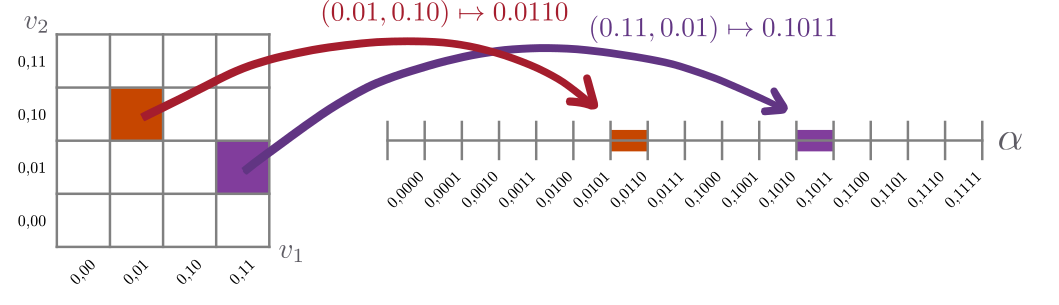
\includegraphics[width=\linewidth]{../figures/S-viz.export.pdf}
[TODO: adapt this figure better, but gives the idea. We see the $4^n$ bins in 2D, and $4^n$ bins in 1D, but twice as many bits]
\endif

% We then loosely have the following correspondence between the discrete connectivity matrices for the one- and two-dimensional neural fields:

% \begin{equation} \begin{aligned}
% \tilde w(\alpha_i,\beta_j) &= \tilde J_{\alpha_i,\beta_j} \\
% &= \tilde J_{S(\vec{v_i},\vec{u_j})} \\
% &= J_{ij} \;\text{by definition} \\
% &= w_U(\vec{v_i},\vec{u_j})
% \end{aligned}\end{equation}

\subsection{Coarse-graining the images to numerically validate the mean-field approximation} \label{sec:coarse-graining}

Coarse-graining adresses the problem of numerically enforcing the mean-field approximation. The mean-field approximation is done on the original two-dimensional neural field when sampling the connectivity matrix $J_{ij}$, as all neurons inside the same grid cells are assumed to be the same. This is not the case when defining the connectivity of the one-dimensional neural field as the permutation of rows and columns of $J_{ij}$.

In order to perform the mean-field approximation on the one-dimensional neural field, we average together $2^n$ consecutive one-dimensional bins, each of length $4^{-n}$, resulting in $2^n$ coarse-grained bins. This is illustrated in Fig. [TODO] Specifically, for every coarse-grained bin $a=1,\cdots,2^n$, the set of consecutive positions $\mathcal{C}_a = \{\tfrac{a-1}{2^n} + \tfrac{l-1}{4^n} \;|\; l \in 1, \cdots, 2^n\}$, gets mapped to the two-dimensional grid points and averaged, intuitively computing the ``center of mass'' of $\mathcal{C}_a$:

\begin{equation*}
\vec{\bar v_a} := \textrm{mean}(\{S^{-1}(\alpha_l) \;|\; \alpha_l \in \mathcal{C}_a\}).
\end{equation*}

\ifndef{SUBMISSION}
\includegraphics[height=15em]{../figures/coarse-graining.pdf}

[TODO: add the indices a,b and l on this figure, for clarity.]
\endif

The obtained coarse-grained points are then used to sample the connectivity kernel, and form the connectivity matrix of the one-dimensional neural field:

\begin{equation} \label{eq:def-tilde-J}
\tilde J_{ab} := w_U(\vec{\bar v_a}, \vec{\bar v_b}).
\end{equation}

\subsection{The cycling gaussian low-rank neural field toy model}

By using the grid-based approach and the coarse-graining procedure, it is now possible to numerically simulate the two-dimensional neural field, and the mapping to the one-dimensional neural field. We introduce a toy model for illustration purposes, but we stress that our results apply to any neural field model.

We extend the model introduced in \cite{schmutz2023convergence}, which can be seen as a simple example of a ``Gaussian mixture low-rank network'' \cite{Beiran2021}. Given the $p$-dimensional embedding $\vec z = (z_1, \cdots, z_p) \in \Rp$, the neural field $h(\vec z, t)$ evolves as:

\begin{equation*} \begin{aligned}
\partial_t h(\vec z, t) &= -h(\vec z, t) + \int_{\Rp} w(\vec z, \vec y) \phi(h(\vec y, t)) \mathcal N^p(\vec y) \mathrm d \vec y, \\
\text{with } w(\vec z, \vec y) &= \sum_{\mu=1}^p z_\mu \tilde\phi(y_\mu) \text{ the connectivity kernel}, \\
\text{where } \tilde\phi(y) &= \frac{\phi(y) - \mathrm E_{y\sim\mathcal N}[\phi(y)]}{\mathrm{Var}_{y\sim\mathcal N}[\phi(y)]}, \quad \mathcal N(y) = \frac{1}{\sqrt{2\pi}} \mathrm{e}^{-\tfrac 12 y^2}, \\
\text{and } \phi(y) &= \frac{1}{1+\mathrm{e}^{-y}}.
\end{aligned} \end{equation*}

The geometric view (see illustation in Fig. [TODO]) of this neural field is that the neuron populations are scattered in a $p$-dimensional Gaussian ball. With the exception of the zero fixed point, there are $p$ ``patterns'' (in this case, the basis functions $f_\mu(\vec z) = z_\mu,\,\mu=1,\cdots,p$) towards which the neural field $h(\vec z,t)$ may converge (we refer to \cite{nvadot2023mathesis}, appendix A for a derivation of the fixed points of this model, and a study of their stability). We stress that one should not confuse the embedding dimension $p$ with the rank of the connectivity kernel, which in this case also coincides with $p$.

\ifndef{SUBMISSION}
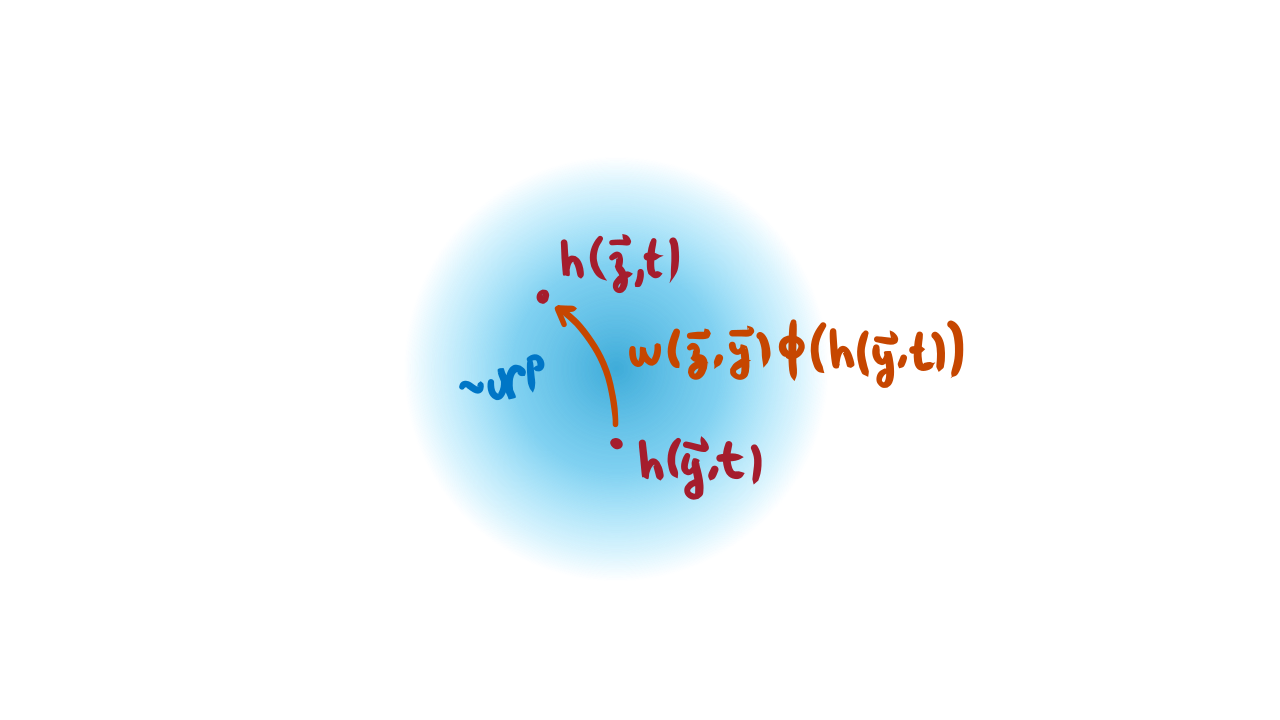
\includegraphics[height=15em]{../figures/lowrankgaussian.pdf}

[TODO: does this need cleaning up (e.g. the Computer Modern font) ?]
\endif

This example is made particularly easy to study, because the kernel and dynamics both have the rank $p$. Firstly, the kernel's low-rank structure makes numerical simulations cheap, as we store $2p$ low-rank vectors of size $4^n$ instead of the full $4^n \times 4^n$ connectivity matrix (see the [TODO: source code url] for the full implementation details). Secondly, by projecting the neural field at any time $t$ onto the $p$ patterns, we can track the full state of the network (setting aside the orthogonal component, which is decoupled and decays exponentially) by following the trajectory in the latent space with the latent variables:
% NOTE: in reality, the latent variables even form a closed system, but this is off-topic for this article

\begin{equation} \label{eq:def-kappa}
\kappa_\mu(t) = \int_{\Rp} y_\mu h(\vec y, t) \mathcal N^p(\vec y) \mathrm d \vec y,\quad \mu=1,\cdots,p.
\end{equation}

To illustrate the latent variables, suppose the neural field has converged to the pattern $h(\vec z, t \to \infty) = z_\mu$. Then the latent variable $\kappa_\mu = 1$, whereas all other latent variables are zero, $\kappa_\mu=0,\,\mu\neq\nu$.

We extend this low-rank Gaussian model by making the dynamics cyclic: instead of converging to a single fixed point, we force the neural field to cycle between the fixed points. This modification makes any differences between numerically evaluated trajectories more apparent, which will be useful when asserting that the dynamics are conserved after the mapping to one dimension. To introduce a cycling behavior, the term $\delta > 0$ ``delays'' the integral term, and the ``rolling'' $z_\mu \mapsto z_{\mu+1}$ (with the convention that $p+1=1$) pushes the recurrent currents to the pattern $\mu+1$ when the neural field is close to the pattern $\mu$. The dynamics of the low-rank Gaussian cycling neural field in \autoref{eq:def-cycling-nf} are illustrated in Fig. [TODO]:

\begin{equation} \label{eq:def-cycling-nf}
\partial_t h(\vec z, t) = -h(\vec z, t) + \int_{\Rp} \sum_{\mu=1}^p z_{\mu+1} \tilde\phi(y_\mu) \phi(h(\vec y, t+\delta)) \mathcal N^p(\vec y) \mathrm d \vec y.
\end{equation}

\ifndef{SUBMISSION}
\includegraphics[width=\linewidth]{../figures/cycling-illustration.png}

[TODO: clean this up]
\endif

\subsection{Simulations of the Column and the Z-mappings applied to the toy model}

In this section, we show numerical simulations of the neural field in $[0,1]$, obtained from applying mappings on higher-dimensional neural fields in $[0,1]^p$. We see that the coarse-graining procedure works when applied from $[0,1]^2$ to $[0,1]$. Then, we demonstrate that it can be applied iteratively, to map from $[0,1]^3$ to $[0,1]^2$, and from $[0,1]^2$ to $[0,1]$.

We start with simulating the cycling neural field \autoref{eq:def-cycling-nf} using the grid-based approach. The connectivity matrix defined in \autoref{eq:def-tilde-J} is computed by applying different mappings to the matrix $J_{ij}$ (that is, permuting the rows and columns), followed by the coarse-graining procedure to reduce to a $2^n \times 2^n$ matrix. Setting $\delta=6$ and the initial condition $h(z_1, z_2, t < 0) = z_1$, simulations are presented in Fig. [TODO] showing the activity levels, recurrent currents, and the latent trajectory $(\kappa_1(t), \kappa_2(t))$. In order, we discuss:
\begin{itemize}
\item The original two-dimensional neural field evolves while oscillating between the patterns $\mu=1$ and $\mu=2$. The neural field is initialized in the $\mu=1$ state, and as a consequence $\kappa_1(0)=1$ and $\kappa_2(0)=0$. The oscillation can better be seen in the latent trajectory $(\kappa_1(t), \kappa_2(t))$, evolving somewhat between the points $(1,0)$ and $(0,1)$.
\item A random mapping can be numerically evaluated as a random permutation of the rows and columns of $J_{ij}$, and is used as the ``worst-case'' example, since all regularity of the original neural field is obviously destroyed. The coarse-graining averages out all the structure of the activity, and the recurrent currents are zero, because the contributions from excitatory and inhibitory populations cancel out. This results in the erasure of the cycling behavior in the latent trajectory, and the latent trajectory stays at $(0,0)$.
\item The Column mapping shows the projection of the initial condition onto the $z_1$ axis, yielding the sigmoidal shape in the $[0,1]$ embedding. Problematically, the current currents corresponding to the pattern $\mu=2$ cancel out and yield zero, and the latent trajectory quickly decays towards $(0,0)$.
\item The Z-mapping shows that despite the fractal structure of the activity, there is still regularity in the $[0,1]$ embedding, resulting in non-zero recurrent currents. In consequence, the latent trajectory shows a clear cycling behavior, that closely matches that of the two-dimensional neural field.
\end{itemize}


\ifndef{SUBMISSION}
\includegraphics[height=30em]{../figures/simulation-snapshots.png}

[TODO: these are simulation snapshots. clean this up, adapt the legends, upload the videos]
\endif

These results suggest that the Z-mapping has the desired properties of conserving the regularity of the original smooth kernel. To further stress this, we demonstrate that we can repeat the dimensionality reduction of the embedding space, by iteratively applying the Z-mapping and coarse-graining. Starting with a three-dimensional neural field (setting $p=3$ in \autoref{eq:def-cycling-nf}), we can simulate the mapping from $[0,1]^3$ to $[0,1]^2$ (by applying, at constant $z_1$, the mapping $Z(z_2,z_3) = \alpha_{23}$), then from $[0,1]^2$ to $[0,1]$ (applying the mapping $Z(\alpha_{23},z_1)=\alpha_{123}$). This is shown in Fig. [TODO], and we assert equivalence of dynamics by studying the numerical equality of the latent trajectories. This demonstrates that for the mapping to yield identical dynamics, the starting kernel only has to be ``continuous on average''.

\ifndef{SUBMISSION}
\includegraphics[height=20em]{../figures/simulation-321-snapshots.png}

[TODO: legend, link video]
\endif

\section{The measure of locality}

In the previous sections we derived the Column and the Z-mapping, and showed that, at least numerically, the Z-mapping seems to be a ``local'' mapping, in the sense that small neighbourhoods in $[0,1]$ are mapped by $S^{-1}$ to small neighbourhoods in $[0,1]^2$. When writing the one-dimensional neural field in \autoref{eq:nf-in-01} with the kernel $\tilde w(\alpha,\beta) = w_U(S^{-1}(\alpha), S^{-1}(\beta))$, are neural populations close in the one-dimensional embedding also close in the two-dimensional embedding?

% TODO: rework this paragraph, i'm tired
% Locality is closely tied to the coarse-graining procedure introduced in \autoref{sec:coarse-graining}, because local mappings will yield populations that are close in $[0,1]^2$, and coarse-graining will not introduce much error; the mean-field approximation is in this case valid. Contrarily, when the mapping is not local, the coarse-graing will average together positions that are far apart, resulting in inaccurate samplings of the connectivity kernel.  For the Column mapping, coarse-graining removes all variation on the vertical axis, reducing the sampling of the kernel $w_U$ to a line: the mapping is not local. The Z-mapping is local: even after coarse-graining, the sampling points span the full two-dimensional as $n \to \infty$.

Locality is closely tied to the coarse-graining procedure introduced in \autoref{sec:coarse-graining}. 
In Fig. [TODO], we colour-code the two-dimensional populations corresponding to the same $\mathcal{C}_a$ before coarse-graining.
We see that the Z-mapping yields populations close in $[0,1]^2$, such that coarse-graining will not introduce much error and the kernel $w_U$ is sampled uniformly as $n \to \infty$: the mean-field approximation for the resulting one-dimensional neural field is valid. On the contrary, the coarse-grained populations of the Column mapping lie on a line in the two-dimensional embedding (it ``changes too fast''), resulting in non-uniform sampling of the kernel $w_U$: this mapping is not local and we cannot properly write the one-dimensional neural field.

\ifndef{SUBMISSION}
\includegraphics[height=20em]{../figures/where-are-the-coarse-grained-positions.png}

[TODO: clean this up]
\endif

\subsection{Definition of locality}

Given $n \in \mathbb N$, let us define the locality $V^n(S^n_\textrm{inv})$ as the average error made by the coarse-graining procedure. For this, we compute the maximum difference in positions of the two-dimensional embedding $\norm{S^n_\textrm{inv}(\alpha) - S^n_\textrm{inv}(\alpha^\prime)}_1$, associated to the one-dimensional populations in the bounds $\left[\tfrac{a-1}{2^n}, \tfrac{a}{2^n}\right]$ of the coarse-graining bin $\mathcal C_a$:

\begin{equation} \label{eq:def-V}
V^n(S^n_\textrm{inv}) = \frac{1}{2^n} \sum_{a=1}^{2^n} \sup_{\alpha, \alpha^\prime \in \left[\frac{a-1}{2^n}, \frac{a}{2^n} \right]} \norm{S^n_\textrm{inv}(\alpha) - S^n_\textrm{inv}(\alpha^\prime)}_1
\end{equation}

Within the context of a sequence of mappings, we are specifically interested in the $n \to \infty$ limit, that is, whether the error of the mean-field approximation vanishes as the grid becomes infinitely fine. For the random, Column and Z-mappings, we graph the scaling behavior of the numerator (the total error of the mean-field approximation) in Fig. [TODO]. As expected, we see that the total error of the Z-mapping scales much slower than $2^n$, whereas that of the Column (and random) mapping scales roughly as $2^n$.

\ifndef{SUBMISSION}
\includegraphics[height=15em]{../figures/locality-scaling.png}

[TODO: cleanup]
\endif

\subsection{Computing the locality of the Column and the Z-mapping}

In this section we analytically derive the locality of the Column and the Z-mapping, showing that $V^n(Z^n_\textrm{inv}) \xrightarrow{n \to \infty} 0$, but that $V^n(C^n_\textrm{inv}) > 0$ for all $n \in \mathbb{N}$.

We consider the binary expansion of $\alpha$ and $\alpha^\prime$ which appear in the supremum of \autoref{eq:def-V}. For clarity of notation, we furthermore truncate the binary expansion to $2m$ bits (on most machines, $2m=64$ bits, but analytically $m$ may be arbitrarily large):

\begin{equation*} \begin{aligned}
\alpha &= 0. b^1 b^2 \cdots b^{2m-1} b^{2m},\\
\alpha^\prime &= 0. b^{\prime 1} b^{\prime 2} \cdots b^{\prime 2m-1} b^{\prime 2m}. \\
\end{aligned} \end{equation*}

Furthermore, since $\alpha \in \left[\frac{i-1}{2^n}, \frac{i}{2^n} \right],\, i \in \{1, \cdots, 2^n\}$, we may express the first $n$ (where $n < 2m$) bits of $\alpha$ with the bits of $i=\sum_{k=0}^{n-1} i^k 2^k$ (ignoring $i=2^n$ for the sake of simplicity, which would introduce one more bit, $n+1$ in total):

\begin{equation*} \begin{aligned}
\alpha &= 0. i^{n-1} i^{n-2} \cdots i^1 i^0 b^n b^{n+1} \cdots b^{2m-1} b^{2m},\\
\alpha^\prime &= 0. i^{n-1} i^{n-2} \cdots i^1 i^0 b^{\prime n} b^{\prime n+1} \cdots b^{\prime 2m-1} b^{\prime 2m}.
\end{aligned} \end{equation*}

\paragraph{Z-mapping.} Let us consider the Z-mapping. If $n$ is even, we write with $\alpha$ defined above (and similarly for $\alpha^\prime$):

$$
\begin{aligned}
Z^n_{\textrm{inv},1}(\alpha) &= 0.\underbrace{i^{n-1} i^{n-3} \cdots i_1}_\text{$n/2$ bits} b^n b^{n+2} \cdots b^{2m-1}, \\
Z^n_{\textrm{inv},2}(\alpha) &= 0.\underbrace{i^{n-2} i^{n-4} \cdots i_0}_\text{$n/2$ bits} b^{n+1} b^{n+3} \cdots b^{2m}.
\end{aligned}
$$

If $n$ is odd, we have:

$$
\begin{aligned}
Z^n_{\textrm{inv},1}(\alpha) &= 0.\underbrace{i^{n-1} i^{n-3} \cdots i^0}_\text{$(n+1)/2$ bits} b^n b^{n+2} \cdots b^{2m-1}, \\
Z^n_{\textrm{inv},2}(\alpha) &= 0.\underbrace{i^{n-2} i^{n-4} \cdots i^1}_\text{$(n-1)/2$ bits} b^{n+1} b^{n+3} \cdots b^{2m}.
\end{aligned}
$$

We only consider even $n$ in the following, as the proof for the latter case remains very similar. The key is that the first $n/2$ bits of the difference of the inverses cancel out:

$$
\begin{aligned}
|Z^n_{\textrm{inv},1}(\alpha) - Z^n_{\textrm{inv},1}(\alpha^\prime)| &= \left|0.0 \cdots 0 (b^n b^{n+2} \cdots b^{2m-1} - b^{\prime n} b^{\prime n+2} \cdots b^{\prime 2m-1})\right| \\
&= \left|2^{-n/2} \sum_{k=1}^{\tfrac{2m-n+1}{2}} (b^{n+2k-1} - b^{\prime n+2k-1}) 2^{-k}\right| \\
&\leq 2^{-n/2} \\
|Z^n_{\textrm{inv},2}(\alpha) - Z^n_{\textrm{inv},2}(\alpha^\prime)| &= \left|2^{-n/2} \sum_{k=1}^{\tfrac{2m-n+1}{2}} (b^{n+2k} - b^{\prime n+2k}) 2^{-k}\right| \\
&\leq 2^{-n/2}
\end{aligned}
$$

Putting everything together, we get the following vanishing upper bound:

$$
V^n(Z^n_\textrm{inv}) \leq \frac{1}{2^n} \sum_{i=1}^{2^n} 2^{-n/2} + 2^{-n/2} = 2^{-n/2+1} \xrightarrow{n \to \infty} 0
$$

\paragraph{Column mapping.} We now consider the Column mapping:

$$
\begin{aligned}
C^n_{\textrm{inv},1}(\alpha) &= 0.i^{n-1} i^{n-2} \cdots i^1 i^0 b^n b^{n+1} \cdots b^m \\
C^n_{\textrm{inv},2}(\alpha) &= 0.b^{m+1} b^{m+2} \cdots b^{2m}.
\end{aligned}
$$

The first component can be bounded using the same trick as for the Z-mapping above:

$$
\begin{aligned}
|C^n_{\textrm{inv},1}(\alpha) - C^n_{\textrm{inv},1}(\alpha^\prime)| &= \left| 2^{-n} \sum_{k=1}^{m-n+1} (b^{n+k-1} - b^{\prime n+k-1}) 2^{-k} \right| \\
&\leq 2^{-n}.
\end{aligned}
$$

However, problems arise due to the second component not being well-behaved. In particular, since we take the supremum on $\alpha,\alpha^\prime \in \left[\tfrac{i-1}{2^n},\tfrac{i}{2^n}\right]^2$, we can pick the specific values such that $b^k=1$ and $b^{\prime k}=0$ for all $k \in \{m+1, \cdots 2m\}$:

$$
\begin{aligned}
|C^n_{\textrm{inv},2}(\alpha) - C^n_{\textrm{inv},2}(\alpha^\prime)| &= \left| \sum_{k=m+1}^{2m} (b^k - b^{\prime k}) 2^{-(k-m)} \right| \\
&= \sum_{k=m+1}^{2m} 2^{-(k-m)} \\
&> \frac 12.
\end{aligned}
$$

Putting both together, we can write:

$$
\begin{aligned}
V^n(C^n_\textrm{inv}) &= \frac{1}{2^n}\sum_{i=1}^{2^n} \sup_{\alpha, \alpha^\prime \in \left[\tfrac{i-1}{2^n}, \tfrac{i}{2^n}\right]^2} |C^n_{\textrm{inv},1}(\alpha^\prime) - C^n_{\textrm{inv},1}(\alpha)| + |C^n_{\textrm{inv},2}(\alpha^\prime) - C^n_{\textrm{inv},2}(\alpha)| \\
&\geq
\begin{aligned}[t]
	\frac{1}{2^n}\sum_{i=1}^{2^n}&
	\sup_{\alpha, \alpha^\prime \in \left[\tfrac{i-1}{2^n}, \tfrac{i}{2^n}\right]^2} |C^n_{\textrm{inv},1}(\alpha^\prime) - C^n_{\textrm{inv},1}(\alpha)|\\
	&+ \sup_{\alpha, \alpha^\prime \in \left[\tfrac{i-1}{2^n}, \tfrac{i}{2^n}\right]^2} |C^n_{\textrm{inv},2}(\alpha^\prime) - C^n_{\textrm{inv},2}(\alpha)|
\end{aligned}\\
&\geq \frac 12 + \bO(2^{-n}).
\end{aligned}
$$

We following upper bound therefore shows that the locality measure cannot converge to zero as $n \to \infty$: 

$$
V^n(C^n_\textrm{inv}) > \frac 12.
$$


\section{Proof of results}

\subsection{Locality garantees convergence of grid-based simulations as $n \to \infty$}.

\subsection{Analytical equivalence given $S$ measurable and bijective}
\label{sec:proof-equivalence}


\section{Conclusion}

% TODO: are all bijective limits local ? does local imply bijection ?
% in this case, we have shown that bijection + locality => we can safely do the mapping (bijection for the analytical approach, locality for the numerical approach)
% TODO: mention the "standard example" of the Z-mapping. This framework is surely not unique, for instance the reclocal bijection cannot easily be expressed as the permutation of bits, but it still works in the same way as the Z-mapping (fractal formulation), and numerical simulations are OK




% Use "Eq" instead of "Equation" for equation citations.
% \section*{Introduction}
% Lorem ipsum dolor sit~\cite{bib1} amet, consectetur adipiscing elit. Curabitur eget porta erat. Morbi consectetur est vel gravida pretium. Suspendisse ut dui eu ante cursus gravida non sed sem. Nullam Eq~(\ref{eq:schemeP}) sapien tellus, commodo id velit id, eleifend volutpat quam. Phasellus mauris velit, dapibus finibus elementum vel, pulvinar non tellus. Nunc pellentesque pretium diam, quis maximus dolor faucibus id.~\cite{bib2} Nunc convallis sodales ante, ut ullamcorper est egestas vitae. Nam sit amet enim ultrices, ultrices elit pulvinar, volutpat risus.

% \begin{eqnarray}
% \label{eq:schemeP}
% 	\mathrm{P_Y} = \underbrace{H(Y_n) - H(Y_n|\mathbf{V}^{Y}_{n})}_{S_Y} + \underbrace{H(Y_n|\mathbf{V}^{Y}_{n})- H(Y_n|\mathbf{V}^{X,Y}_{n})}_{T_{X\rightarrow Y}},
% \end{eqnarray}

% \section*{Materials and methods}
% \subsection*{Etiam eget sapien nibh}

% % For figure citations, please use "Fig" instead of "Figure".
% Nulla mi mi, Fig~\ref{fig1} venenatis sed ipsum varius, volutpat euismod diam. Proin rutrum vel massa non gravida. Quisque tempor sem et dignissim rutrum. Lorem ipsum dolor sit amet, consectetur adipiscing elit. Morbi at justo vitae nulla elementum commodo eu id massa. In vitae diam ac augue semper tincidunt eu ut eros. Fusce fringilla erat porttitor lectus cursus, \nameref{S1_Video} vel sagittis arcu lobortis. Aliquam in enim semper, aliquam massa id, cursus neque. Praesent faucibus semper libero.

% % Place figure captions after the first paragraph in which they are cited.
% \begin{figure}[!h]
% \caption{{\bf Bold the figure title.}
% Figure caption text here, please use this space for the figure panel descriptions instead of using subfigure commands. A: Lorem ipsum dolor sit amet. B: Consectetur adipiscing elit.}
% \label{fig1}
% \end{figure}

% % Results and Discussion can be combined.
% \section*{Results}
% Nulla mi mi, venenatis sed ipsum varius, Table~\ref{table1} volutpat euismod diam. Proin rutrum vel massa non gravida. Quisque tempor sem et dignissim rutrum. Lorem ipsum dolor sit amet, consectetur adipiscing elit. Morbi at justo vitae nulla elementum commodo eu id massa. In vitae diam ac augue semper tincidunt eu ut eros. Fusce fringilla erat porttitor lectus cursus, vel sagittis arcu lobortis. Aliquam in enim semper, aliquam massa id, cursus neque. Praesent faucibus semper libero.

% % Place tables after the first paragraph in which they are cited.
% \begin{table}[!ht]
% \begin{adjustwidth}{-2.25in}{0in} % Comment out/remove adjustwidth environment if table fits in text column.
% \centering
% \caption{
% {\bf Table caption Nulla mi mi, venenatis sed ipsum varius, volutpat euismod diam.}}
% \begin{tabular}{|l+l|l|l|l|l|l|l|}
% \hline
% \multicolumn{4}{|l|}{\bf Heading1} & \multicolumn{4}{|l|}{\bf Heading2}\\ \thickhline
% $cell1 row1$ & cell2 row 1 & cell3 row 1 & cell4 row 1 & cell5 row 1 & cell6 row 1 & cell7 row 1 & cell8 row 1\\ \hline
% $cell1 row2$ & cell2 row 2 & cell3 row 2 & cell4 row 2 & cell5 row 2 & cell6 row 2 & cell7 row 2 & cell8 row 2\\ \hline
% $cell1 row3$ & cell2 row 3 & cell3 row 3 & cell4 row 3 & cell5 row 3 & cell6 row 3 & cell7 row 3 & cell8 row 3\\ \hline
% \end{tabular}
% \begin{flushleft} Table notes Phasellus venenatis, tortor nec vestibulum mattis, massa tortor interdum felis, nec pellentesque metus tortor nec nisl. Ut ornare mauris tellus, vel dapibus arcu suscipit sed.
% \end{flushleft}
% \label{table1}
% \end{adjustwidth}
% \end{table}


% %PLOS does not support heading levels beyond the 3rd (no 4th level headings).
% \subsection*{\lorem\ and \ipsum\ nunc blandit a tortor}
% \subsubsection*{3rd level heading} 
% Maecenas convallis mauris sit amet sem ultrices gravida. Etiam eget sapien nibh. Sed ac ipsum eget enim egestas ullamcorper nec euismod ligula. Curabitur fringilla pulvinar lectus consectetur pellentesque. Quisque augue sem, tincidunt sit amet feugiat eget, ullamcorper sed velit. Sed non aliquet felis. Lorem ipsum dolor sit amet, consectetur adipiscing elit. Mauris commodo justo ac dui pretium imperdiet. Sed suscipit iaculis mi at feugiat. 

% \begin{enumerate}
% 	\item{react}
% 	\item{diffuse free particles}
% 	\item{increment time by dt and go to 1}
% \end{enumerate}


% \subsection*{Sed ac quam id nisi malesuada congue}

% Nulla mi mi, venenatis sed ipsum varius, volutpat euismod diam. Proin rutrum vel massa non gravida. Quisque tempor sem et dignissim rutrum. Lorem ipsum dolor sit amet, consectetur adipiscing elit. Morbi at justo vitae nulla elementum commodo eu id massa. In vitae diam ac augue semper tincidunt eu ut eros. Fusce fringilla erat porttitor lectus cursus, vel sagittis arcu lobortis. Aliquam in enim semper, aliquam massa id, cursus neque. Praesent faucibus semper libero.

% \begin{itemize}
% 	\item First bulleted item.
% 	\item Second bulleted item.
% 	\item Third bulleted item.
% \end{itemize}

% \section*{Discussion}
% Nulla mi mi, venenatis sed ipsum varius, Table~\ref{table1} volutpat euismod diam. Proin rutrum vel massa non gravida. Quisque tempor sem et dignissim rutrum. Lorem ipsum dolor sit amet, consectetur adipiscing elit. Morbi at justo vitae nulla elementum commodo eu id massa. In vitae diam ac augue semper tincidunt eu ut eros. Fusce fringilla erat porttitor lectus cursus, vel sagittis arcu lobortis. Aliquam in enim semper, aliquam massa id, cursus neque. Praesent faucibus semper libero~\cite{bib3}.

% \section*{Conclusion}

% CO\textsubscript{2} Maecenas convallis mauris sit amet sem ultrices gravida. Etiam eget sapien nibh. Sed ac ipsum eget enim egestas ullamcorper nec euismod ligula. Curabitur fringilla pulvinar lectus consectetur pellentesque. Quisque augue sem, tincidunt sit amet feugiat eget, ullamcorper sed velit. 

% Sed non aliquet felis. Lorem ipsum dolor sit amet, consectetur adipiscing elit. Mauris commodo justo ac dui pretium imperdiet. Sed suscipit iaculis mi at feugiat. Ut neque ipsum, luctus id lacus ut, laoreet scelerisque urna. Phasellus venenatis, tortor nec vestibulum mattis, massa tortor interdum felis, nec pellentesque metus tortor nec nisl. Ut ornare mauris tellus, vel dapibus arcu suscipit sed. Nam condimentum sem eget mollis euismod. Nullam dui urna, gravida venenatis dui et, tincidunt sodales ex. Nunc est dui, sodales sed mauris nec, auctor sagittis leo. Aliquam tincidunt, ex in facilisis elementum, libero lectus luctus est, non vulputate nisl augue at dolor. For more information, see \nameref{S1_Appendix}.

% \section*{Supporting information}

% % Include only the SI item label in the paragraph heading. Use the \nameref{label} command to cite SI items in the text.
% \paragraph*{S1 Fig.}
% \label{S1_Fig}
% {\bf Bold the title sentence.} Add descriptive text after the title of the item (optional).

% \paragraph*{S2 Fig.}
% \label{S2_Fig}
% {\bf Lorem ipsum.} Maecenas convallis mauris sit amet sem ultrices gravida. Etiam eget sapien nibh. Sed ac ipsum eget enim egestas ullamcorper nec euismod ligula. Curabitur fringilla pulvinar lectus consectetur pellentesque.

% \paragraph*{S1 File.}
% \label{S1_File}
% {\bf Lorem ipsum.}  Maecenas convallis mauris sit amet sem ultrices gravida. Etiam eget sapien nibh. Sed ac ipsum eget enim egestas ullamcorper nec euismod ligula. Curabitur fringilla pulvinar lectus consectetur pellentesque.

% \paragraph*{S1 Video.}
% \label{S1_Video}
% {\bf Lorem ipsum.}  Maecenas convallis mauris sit amet sem ultrices gravida. Etiam eget sapien nibh. Sed ac ipsum eget enim egestas ullamcorper nec euismod ligula. Curabitur fringilla pulvinar lectus consectetur pellentesque.

% \paragraph*{S1 Appendix.}
% \label{S1_Appendix}
% {\bf Lorem ipsum.} Maecenas convallis mauris sit amet sem ultrices gravida. Etiam eget sapien nibh. Sed ac ipsum eget enim egestas ullamcorper nec euismod ligula. Curabitur fringilla pulvinar lectus consectetur pellentesque.

% \paragraph*{S1 Table.}
% \label{S1_Table}
% {\bf Lorem ipsum.} Maecenas convallis mauris sit amet sem ultrices gravida. Etiam eget sapien nibh. Sed ac ipsum eget enim egestas ullamcorper nec euismod ligula. Curabitur fringilla pulvinar lectus consectetur pellentesque.

% \section*{Acknowledgments}
% Cras egestas velit mauris, eu mollis turpis pellentesque sit amet. Interdum et malesuada fames ac ante ipsum primis in faucibus. Nam id pretium nisi. Sed ac quam id nisi malesuada congue. Sed interdum aliquet augue, at pellentesque quam rhoncus vitae.

\nolinenumbers

% Either type in your references using
% \begin{thebibliography}{}
% \bibitem{}
% Text
% \end{thebibliography}
%
% or
%
% Compile your BiBTeX database using our plos2015.bst
% style file and paste the contents of your .bbl file
% here. See http://journals.plos.org/plosone/s/latex for 
% step-by-step instructions.
% 

% bibliography automatically substituted by gpp preprocessor,
% run `make` (see also: Makefile)
\ifdef{SUBMISSION}\include{"manuscript-tmp.bbl"}\else\bibliography{references}\endif

\end{document}

